\section{Chi tiết về Đồ án}

\subsection{Đồ họa và các chức năng cơ bản}

\subsubsection{Title}
Màn hình chính gồm các cửa sổ nhỏ trong trò chơi, bao gồm các cửa sổ như "New Game", "Load Game", "About" và "Help". Khi người chơi điều hướng đến từng cửa sổ, các ô trong giao diện sẽ thay đổi màu sắc tương ứng.
\begin{figure}[H]
    \centering
    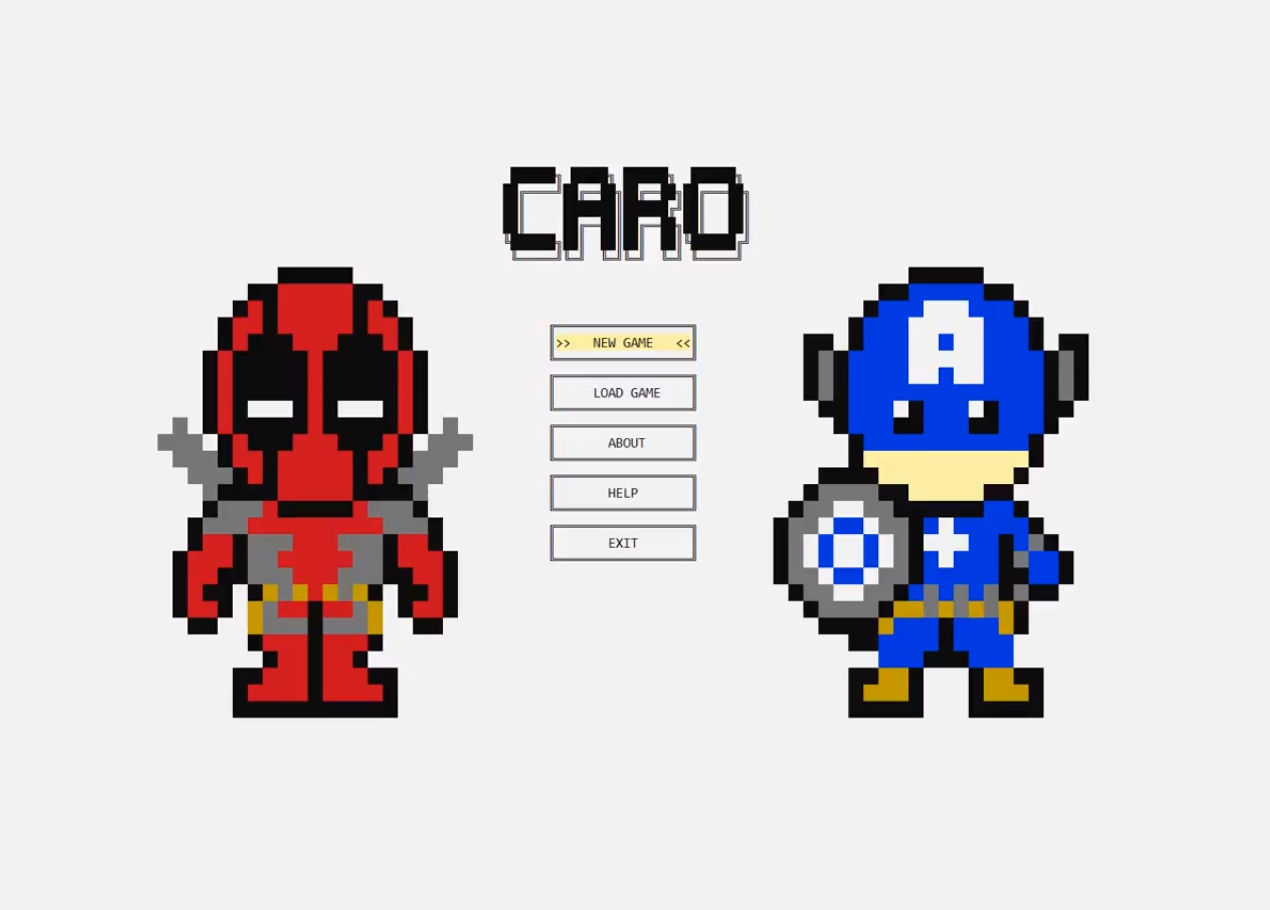
\includegraphics[scale=.5]{img/title.png}
    \caption{Title (updated 17/11/2023)}
\end{figure}
\clearpage
\subsubsection{New Game}
Trong cửa sổ nhỏ New Game, có 2 chế độ để người chơi lựa chọn:
\begin{itemize}
    \item Chơi với máy (1 Player)
    \item Hai người chơi (2 Players)
\end{itemize}
\begin{figure}[H]
    \centering
    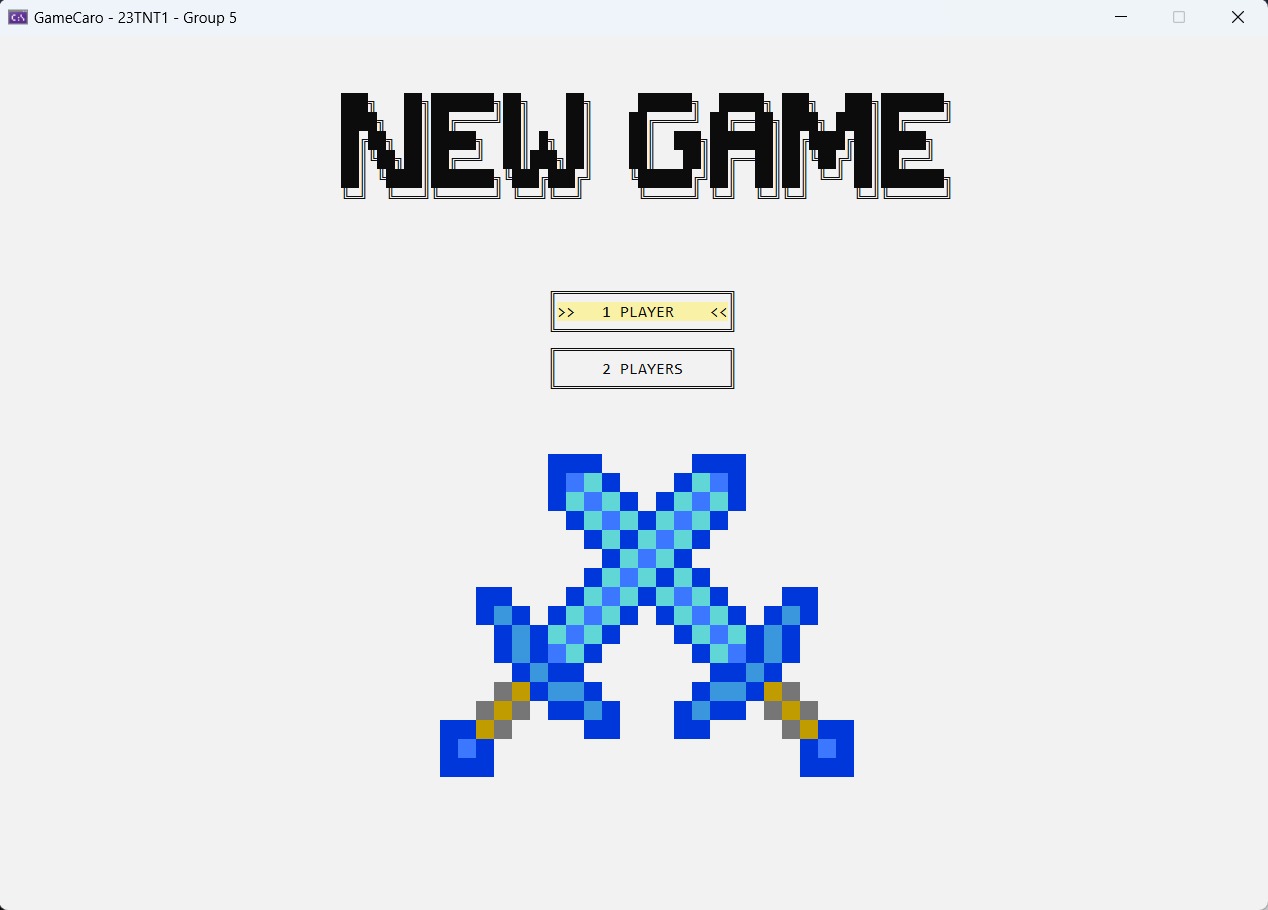
\includegraphics[scale=.4]{img/newgame.png}
    \caption{New Game (updated 17/11/2023)}
\end{figure}
\clearpage
\subsubsection{In match}
Người chơi có thể di chuyển bằng các nút trên bàn phím. Trong quá trình chơi, biểu tượng X và O sẽ thay đổi màu sắc để thông báo lượt đi. Khi phân định thắng-thua, dòng liên tiếp 5 ô X hoặc O sẽ nhấp nháy và kết quả sẽ được hiển thị qua hộp thoại với thông báo "X WIN" hoặc "O WIN". Người chơi cũng có thể lựa chọn các chế độ như "Exit Game" (Esc), "Undo" (U) và "Save Game" (I) trong quá trình chơi.
\begin{figure}[H]
    \centering
    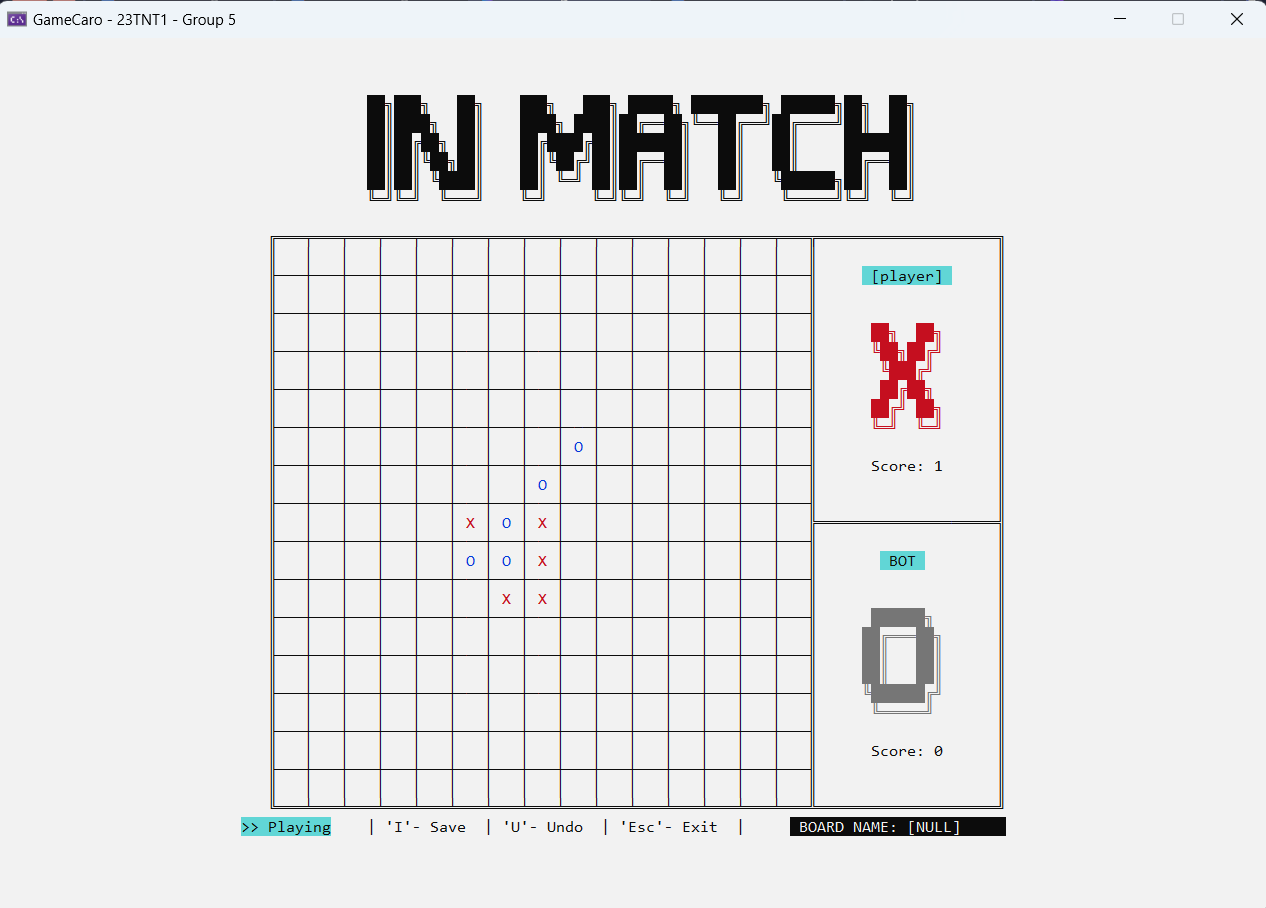
\includegraphics[scale=.4]{img/inmatch.png}
    \caption{In Match (updated 17/11/2023)}
\end{figure}
\clearpage
\subsubsection{Load Game}
Có tổng cộng 15 file trống được cung cấp cho người chơi để thuận tiện trong việc lưu trữ. Mỗi file có một tên và độ dài tên nhất định. Khi người chơi chọn một file đã lưu, họ sẽ có một loạt các lựa chọn, bao gồm "PLAY" (để quay lại màn hình chính và tiếp tục chơi), "DELETE" (để xóa file đã lưu) hoặc "RENAME" (để đổi tên file nếu người chơi muốn thay đổi tên).
\begin{figure}[H]
    \centering
    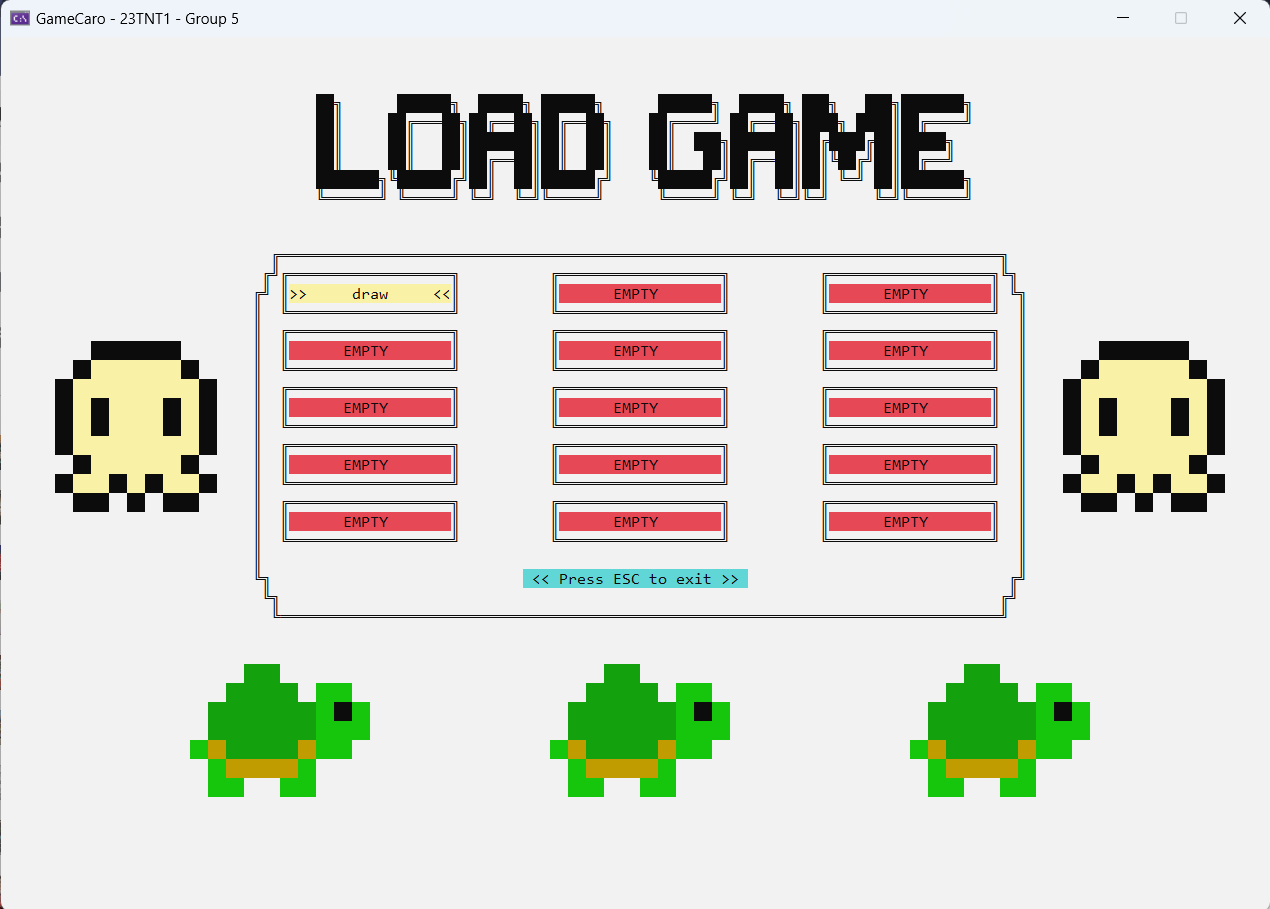
\includegraphics[scale=.4]{img/loadgame.png}
    \caption{Load Game (updated 17/11/2023)}
\end{figure}
\clearpage
\subsubsection{Help}
Phần Help có các hướng dẫn cơ bản cho người chơi.
\begin{figure}[H]
    \centering
    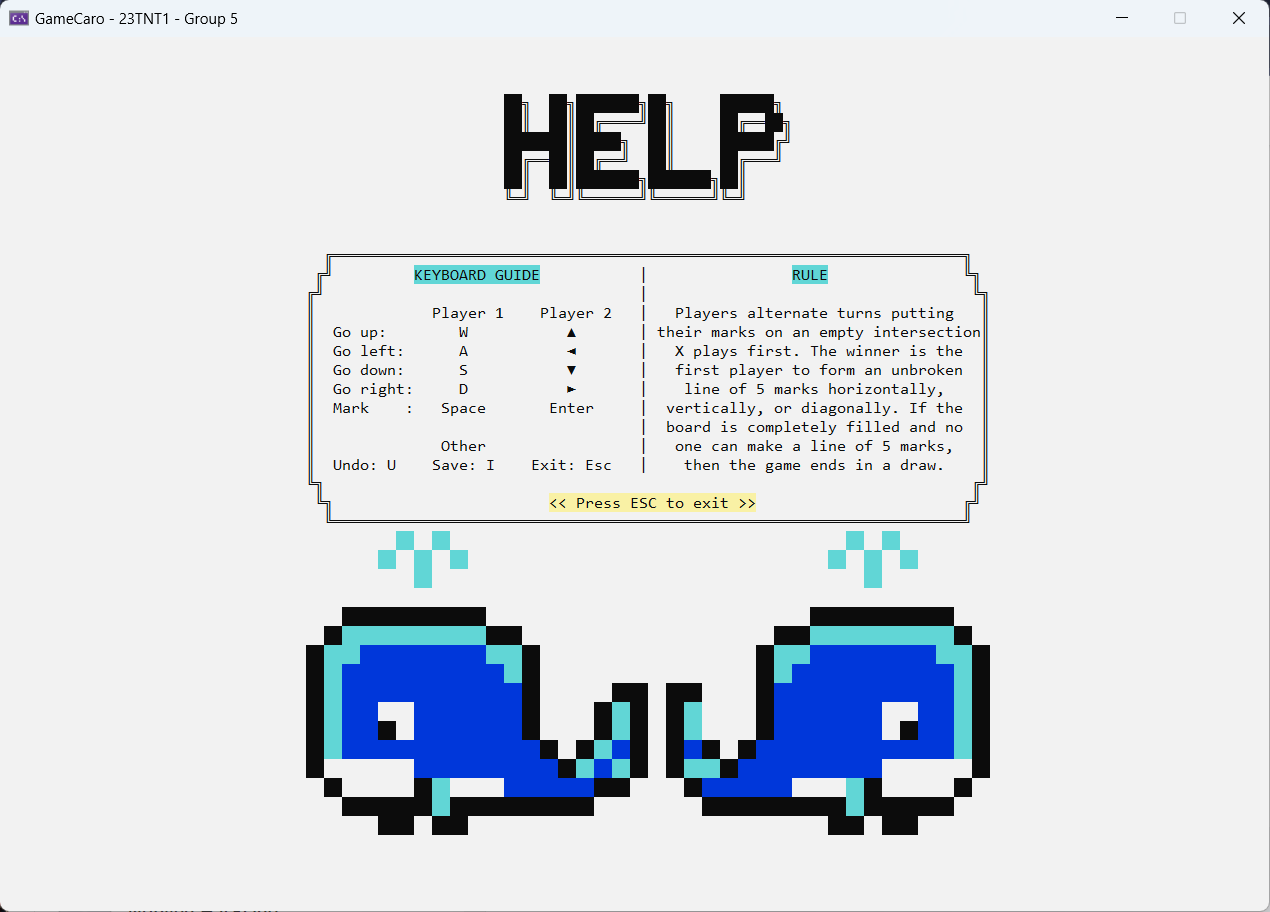
\includegraphics[scale=.4]{img/help.png}
    \caption{Help (updated 17/11/2023)}
\end{figure}
\clearpage
\subsubsection{About}
Phần About gồm thông tin thành viên nhóm và giảng viên hướng dẫn.
\begin{figure}[H]
    \centering
    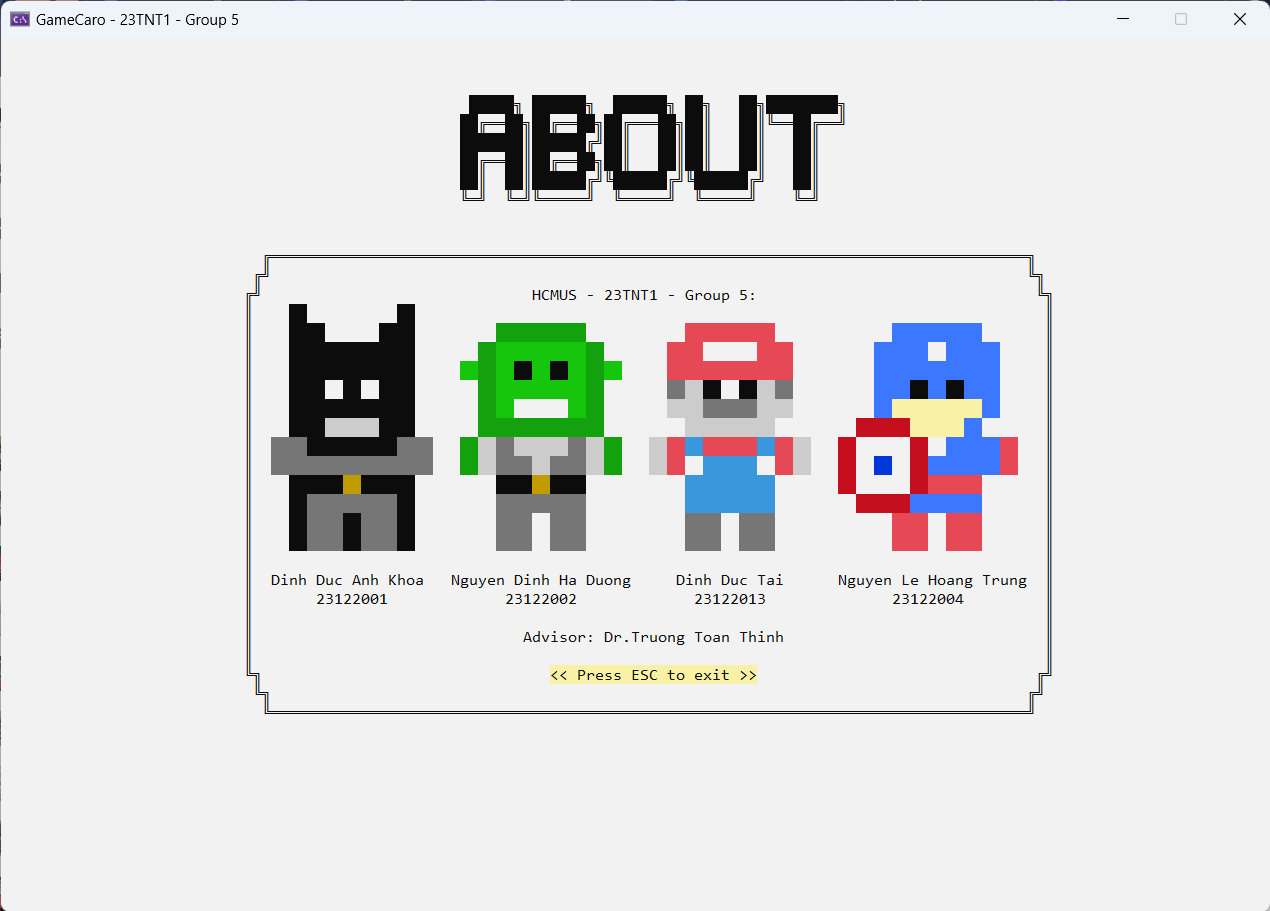
\includegraphics[scale=.4]{img/about.png}
    \caption{About (updated 17/11/2023)}
\end{figure}
\clearpage
\subsection{Thuật toán - Hệ thống trò chơi}
Đây là những chức năng đã được xây dựng thành công, cùng với một phần thuật toán để minh họa:
\subsubsection{Minimax, Alpha-Beta Pruning}
Xây dựng thuật toán AI dành cho chế độ 1 người chơi : Thuật toán Minimax, thuật toán cắt tỉa Alpha-Beta
\lstinputlisting[language=C++]{code/minimax.cpp}
\subsubsection{Điều khiển bằng bàn phím}
Người chơi có thể điều khiển bằng các phím AWDS, các phím mũi tên cùng các phím khác như I, U, Space, Esc,... để tương tác với trò chơi.
\lstinputlisting[language=C++]{code/keyboard.cpp}
\subsubsection{Lưu và chơi tiếp game}
Vào cửa sổ nhỏ Load Game để chơi tiếp trò chơi đã lưu. Trong khi chơi, có thể lưu lại game.
\lstinputlisting[language=C++]{code/saveload.cpp}
\subsubsection{Phân định thắng thua}
Khi hoàn thành trò chơi,hệ thống sẽ phân định thắng thua giữa hai người chơi. 
\lstinputlisting[language=C++]{code/winlose.cpp}
\subsubsection{2 chế độ chơi}
Có 2 chế độ : Đấu với Bot hoặc đấu với người.


